\documentclass[12pt,a4paper]{article}
\usepackage[utf8]{inputenc}
\usepackage[spanish,es-tabla]{babel}
\usepackage{geometry}
\usepackage{graphicx}
\usepackage{multirow}
\usepackage{tabularx}
\usepackage{mathptmx}
\usepackage{fancyhdr}
\usepackage{array}
\usepackage[table]{xcolor}
\usepackage{titlesec}
\usepackage{setspace}
\usepackage{microtype}
\usepackage{lastpage}
\usepackage{booktabs}
\usepackage{enumitem}
\usepackage{amsmath}
\usepackage{amsfonts}
\usepackage{amssymb}

\graphicspath{{images/}{../images/}{./}}

\geometry{
    top=4.7cm,
    bottom=2.5cm,
    left=2.5cm,
    right=2.5cm,
    headheight=3.9cm,
    headsep=0.4cm
}

\setstretch{1.15}
\setlength{\parindent}{0pt}
\setlength{\parskip}{0.45em}
\setlength{\tabcolsep}{4pt}

\titleformat{\section}
  {\normalfont\fontsize{12}{14.5}\bfseries}{\thesection.}{0.6em}{\uppercase}
\titlespacing*{\section}
  {0pt}{1.8ex plus 0.4ex minus 0.2ex}{0.6ex plus 0.2ex}

\titleformat{\subsection}
  {\normalfont\fontsize{11.5}{13.5}\bfseries}{\thesubsection.}{0.5em}{}
\titlespacing*{\subsection}
  {0pt}{1.4ex plus 0.3ex minus 0.1ex}{0.4ex plus 0.1ex}

\titleformat{\subsubsection}
  {\normalfont\fontsize{10.5}{12.5}\bfseries\itshape}{\thesubsubsection.}{0.4em}{}
\titlespacing*{\subsubsection}
  {0pt}{1.1ex plus 0.2ex minus 0.1ex}{0.3ex plus 0.1ex}

\newcolumntype{Y}{>{\centering\arraybackslash}X}
\newcolumntype{L}{>{\raggedright\arraybackslash}X}
\newcolumntype{C}{>{\centering\arraybackslash}X}

\definecolor{headerred}{RGB}{180, 0, 0}
\definecolor{darkred}{RGB}{140, 0, 0}
\definecolor{lightgraybg}{RGB}{248, 248, 248}
\definecolor{tableheader}{RGB}{232, 238, 246}

\newcommand{\docCodigo}{TI-SIGE-ENT-S1-006}
\newcommand{\docVersion}{1.0}
\newcommand{\docProceso}{GESTIÓN FINANCIERA Y EVALUACIÓN DE PROYECTOS}
\newcommand{\docElaboracion}{24/08/2026}
\newcommand{\docRevision}{PENDIENTE DE REVISIÓN}
\newcommand{\docTitulo}{CASO DE NEGOCIO (BUSINESS CASE), COSTOS Y RETORNO DE INVERSIÓN (ROI)}
\newcommand{\docOrganizacion}{FACULTAD DE INGENIERÍA EN SISTEMAS, ELECTRÓNICA E INDUSTRIAL}
\newcommand{\docSubOrganizacion}{CARRERA DE INGENIERÍA DE SOFTWARE}

\newcommand{\encabezadofrecuente}{%
    \renewcommand{\arraystretch}{1.15}%
    \noindent\makebox[\textwidth][c]{%
    \begin{tabularx}{\textwidth}{|>{\centering\arraybackslash}m{2.8cm}|Y|>{\centering\arraybackslash}m{4.8cm}|}
        \hline
        \multirow{4}{2.8cm}{\centering\raisebox{-1.15cm}{
\includegraphics[width=2.5cm,height=2.0cm,keepaspectratio]{images/logo.png}}}
        & \textbf{\fontsize{9}{11}\selectfont \docOrganizacion} 
        & \textbf{\fontsize{8}{10}\selectfont CÓDIGO:} \fontsize{8}{10}\selectfont \docCodigo \\
        \cline{3-3}
        & \textbf{\fontsize{8.5}{10.5}\selectfont \docSubOrganizacion} 
        & \textbf{\fontsize{8}{10}\selectfont VERSIÓN:} \fontsize{8}{10}\selectfont \docVersion \\
        \cline{2-3}
        & \textbf{\fontsize{8}{10}\selectfont PROCESO:} \fontsize{8}{10}\selectfont \docProceso 
        & \textbf{\fontsize{8}{10}\selectfont ELABORACIÓN:} \fontsize{8}{10}\selectfont \docElaboracion \\
        \cline{2-3}
        & \textbf{\fontsize{8.5}{10.5}\selectfont \docTitulo} 
        & \textbf{\fontsize{8}{10}\selectfont ÚLTIMA REVISIÓN:} \fontsize{8}{10}\selectfont \textbf{\textcolor{darkred}{\docRevision}} \\
        \hline
    \end{tabularx}%
    }%
}

\pagestyle{fancy}
\fancyhf{}
\fancyhead[C]{\encabezadofrecuente}
\fancyfoot[C]{\fontsize{10}{12}\selectfont Página \thepage\ de \pageref{LastPage}}
\renewcommand{\headrulewidth}{0pt}

\begin{document}

\section{Título}
\textbf{Denominación del Entregable:} Caso de Negocio, Análisis Costo-Beneficio (ROI, Payback) y Matriz de Riesgos (EDT 1.6)

\vspace{0.15cm}
\noindent
\textbf{Ficha Técnica de Identificación:}
\begin{itemize}[leftmargin=1.5em, itemsep=1.5pt, topsep=1.5pt]
    \item \textbf{Código Documental:} \docCodigo \quad | \quad \textbf{Versión:} \docVersion
    \item \textbf{Institución:} Universidad Técnica de Ambato (UTA) -- FISEI
    \item \textbf{Carrera:} Ingeniería de Software (Séptimo Semestre "A")
    \item \textbf{Módulo Académico:} Gestión de Proyectos de Software
    \item \textbf{Docente Tutor:} Ing. Paulo Torres
    \item \textbf{Fecha de Elaboración:} \docElaboracion \quad | \quad \textbf{Estado:} \textbf{\textcolor{darkred}{En Elaboración / Pendiente de Revisión}}
    \item \textbf{Período de Ejecución:} Semana 1 (21/08/2026 al 24/08/2026)
    \item \textbf{Responsables:} Steeven Toala, Heidy Villavicencio, Nixon Hurtado, Andrea Vasquez
\end{itemize}

\section{Introducción}
La viabilidad de una inversión en tecnologías de información requiere una justificación cuantitativa y estratégica rigurosa. En este documento se presenta el \textbf{Caso de Negocio} para la implantación del sistema \textbf{SIGE}, fundamentado en la reducción de costos operativos por eliminación de papel, optimización del tiempo de revisión docente y mitigación de riesgos de auditoría del Sistema de Gestión de Calidad (SGC).

\subsection{Situación Actual (As-Is)}
Actualmente, la planificación y rendición de cuentas de la planta docente de la FISEI se realiza mediante documentos de texto estáticos y hojas de cálculo independientes. Este proceso manual genera dispersión documental en correos institucionales, extravío de evidencias probatorias, errores aritméticos en matrices de actividades y sobrecarga administrativa que consume en promedio \textbf{8 horas de trabajo por informe}.

\subsection{Oportunidad de Innovación}
La implantación de la plataforma web \textbf{SIGE} transformará este proceso en un flujo digital, estructurado, transparente e inteligente, estandarizando los formatos oficiales vigentes de planes e informes del SGC, automatizando el control de evidencias mediante \textbf{MinIO S3} y asistiendo al docente con \textbf{IA híbrida (corrector LanguageTool en Docker local y asistencia semántica con Google Gemini API)}.

\section{Objetivo}

\subsection{Objetivo General}
Demostrar la viabilidad financiera, técnica, operativa y legal del desarrollo e implantación de SIGE en la FISEI mediante indicadores cuantitativos formalizados (ROI, Payback, Ahorro Anual de Horas).

\subsection{Objetivos Específicos}
\begin{enumerate}[leftmargin=1.5em, itemsep=2pt, topsep=2pt]
    \item Cuantificar la inversión directa en infraestructura cloud requerida (\$630.30 USD).
    \item Proyectar los ahorros operacionales anuales por recuperación de tiempo docente (\$22,500.00 USD) y eliminación de impresiones (\$1,200.00 USD).
    \item Evaluar el Retorno de Inversión (+3,660.0\%) y el período de recuperación (9.7 días).
    \item Construir la matriz de mitigación para los 5 riesgos clave del proyecto.
\end{enumerate}

\section{Alcance}

\subsection{Límites del Análisis (In-Scope)}
\begin{itemize}[leftmargin=1.5em, itemsep=2pt]
    \item Evaluación económica sobre una población estimada de 120 docentes de la facultad durante 2 ciclos académicos anuales.
    \item Costos de infraestructura computacional (servidor VPS, PostgreSQL gestionado, MinIO S3, dominio, SSL, SMTP).
\end{itemize}

\subsection{Exclusiones (Out-of-Scope)}
\begin{itemize}[leftmargin=1.5em, itemsep=2pt]
    \item No monetiza beneficios intangibles como el incremento en la reputación institucional en procesos de acreditación nacional (CACES).
\end{itemize}

\section{Definiciones}
\begin{itemize}[leftmargin=1.5em, itemsep=2pt]
    \item \textbf{ROI (\textit{Return on Investment}):} Indicador porcentual que mide la rentabilidad del proyecto frente a la inversión inicial.
    \item \textbf{Payback:} Período temporal necesario para recuperar el capital invertido mediante los ahorros netos generados.
    \item \textbf{CAPEX (\textit{Capital Expenditure}):} Gastos de capital asociados a la inversión directa inicial.
    \item \textbf{OPEX (\textit{Operational Expenditure}):} Costos recurrentes de operación y mantenimiento de la infraestructura.
\end{itemize}

\section{Responsabilidades}
\begin{table}[htbp]
\centering
\small
\begin{tabularx}{\textwidth}{|>{\hsize=0.6\hsize\bfseries}X|>{\hsize=0.9\hsize}X|>{\hsize=1.5\hsize}X|}
    \hline
    \rowcolor{tableheader}
    Integrante & Rol en el Entregable & Responsabilidad Específica \\
    \hline
    Andrea Vasquez & Frontend / QA & Proyección de ahorros en tiempo de usuario y análisis comparativo de costos. \\
    \hline
    Steeven Toala & Líder de Proyecto / Arquitecto & Costeo de infraestructura cloud, fórmulas de ROI y matriz de riesgos. \\
    \hline
    Heidy Villavicencio & Analista de Requerimientos & Evaluación del impacto organizacional en docentes y comisiones. \\
    \hline
    Nixon Hurtado & Backend / DBA & Estimación de consumo de base de datos y almacenamiento S3. \\
    \hline
    Ing. Paulo Torres & Docente Tutor & Validación y aprobación del modelo financiero y supuestos económicos. \\
    \hline
\end{tabularx}
\caption{Matriz de Responsabilidades del Entregable EDT 1.6.}
\end{table}

\section{Normativa Legal y Técnica}
\begin{itemize}[leftmargin=1.5em, itemsep=2pt]
    \item \textbf{Metodología de Evaluación de Proyectos de Inversión (CEPAL/BID):} Criterios de evaluación costo-beneficio.
    \item \textbf{Ley Orgánica de Educación Superior (LOES):} Principio de eficiencia y optimización de recursos públicos.
    \item \textbf{Manual de Calidad SGC UTA:} Directrices de rendición de cuentas institucional.
\end{itemize}

\section{Método, Políticas y Contenidos}
El análisis financiero se estructura a partir de la cuantificación de horas hombre ahorradas y la eliminación de suministros físicos:

\begin{figure}[htbp]
    \centering
    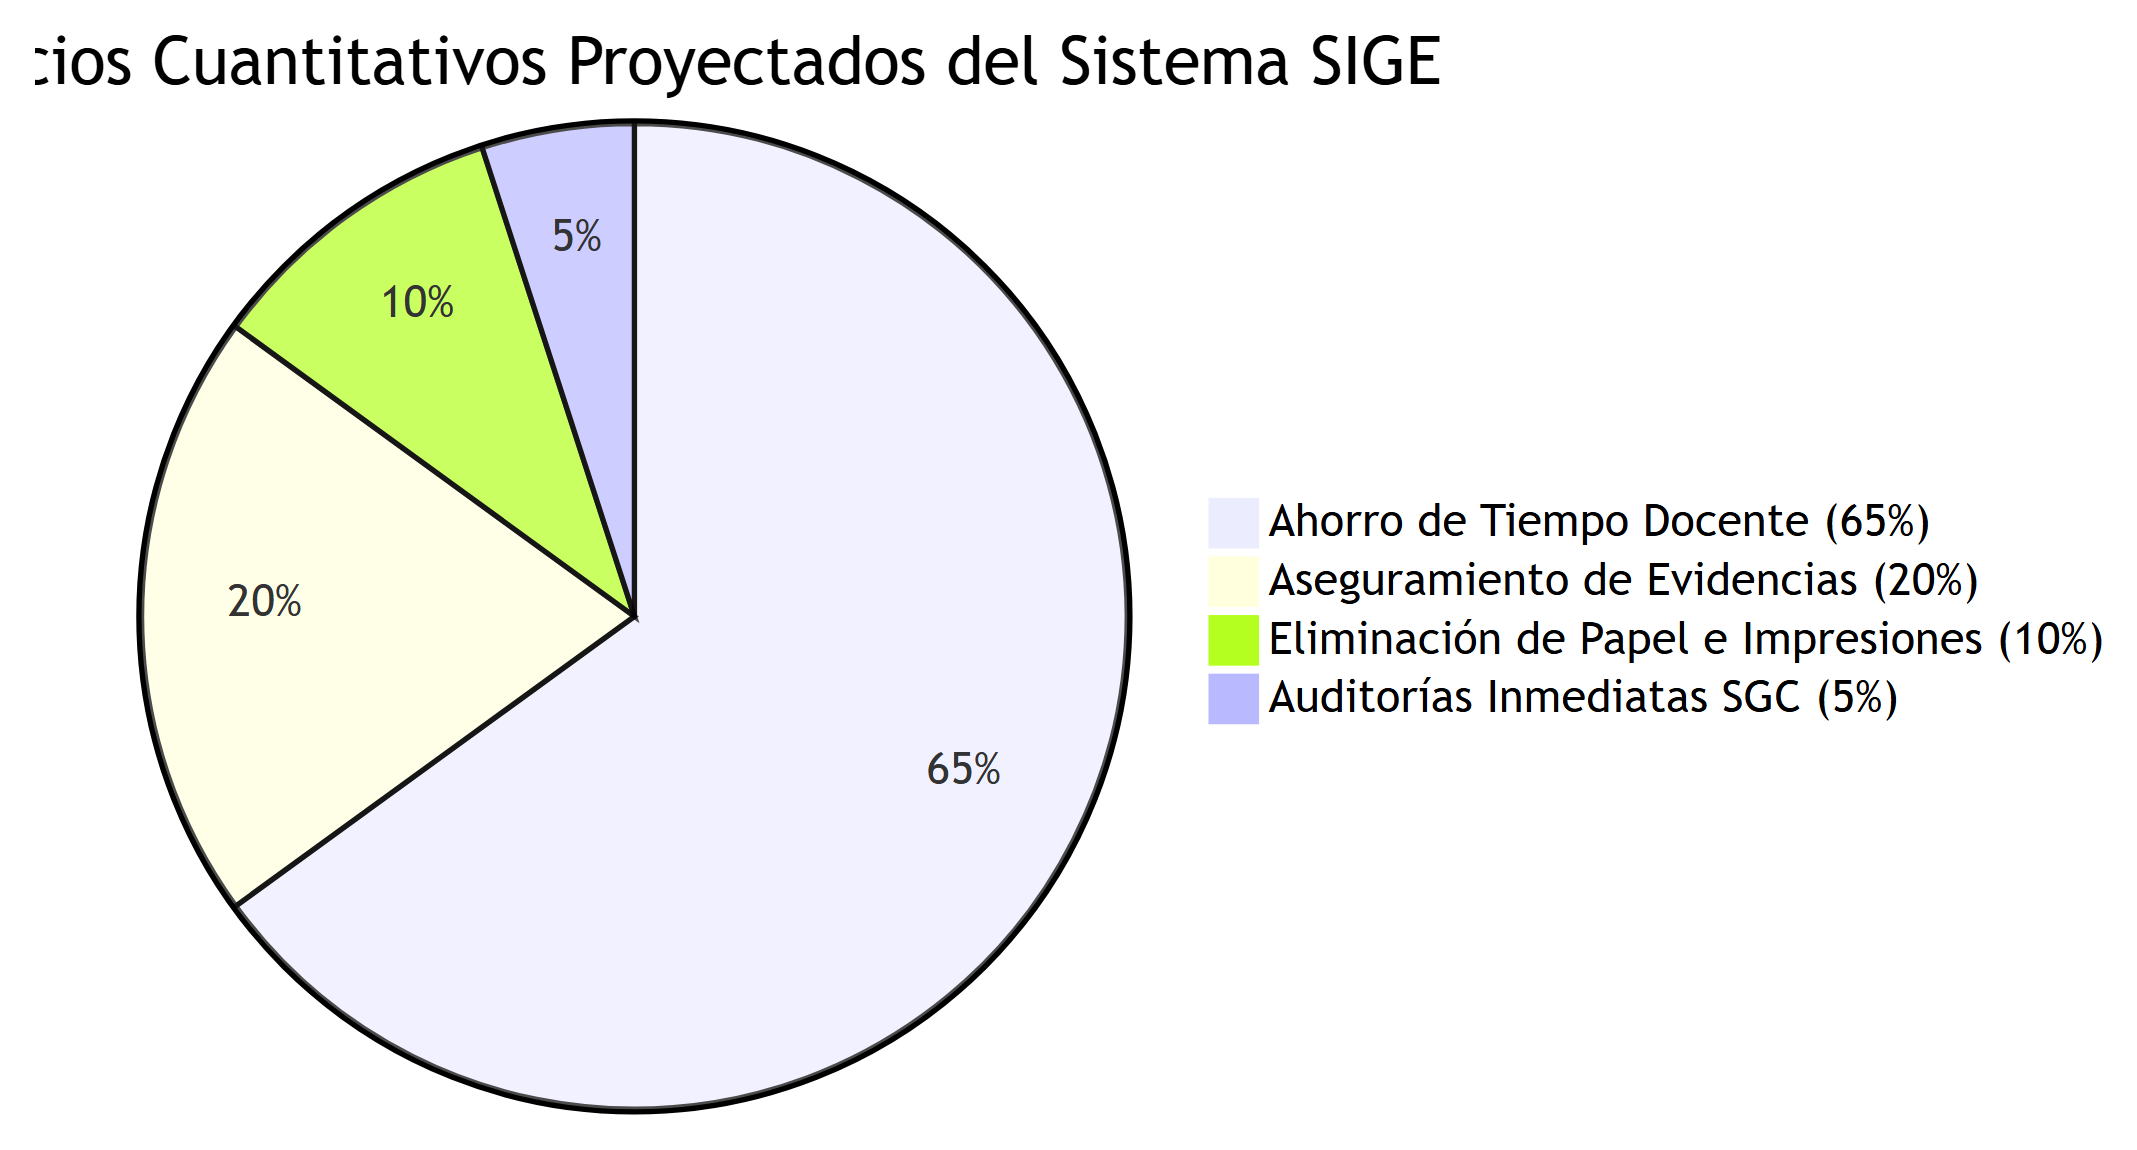
\includegraphics[width=0.72\textwidth,height=5.2cm,keepaspectratio]{images/s1_06_beneficios_pie.png}
    \caption{Distribución de Beneficios Cuantitativos Proyectados del Sistema SIGE.}
    \label{fig:s1_06_pie}
\end{figure}

\begin{enumerate}[leftmargin=1.5em, itemsep=2pt]
    \item \textbf{Reducción del 65\% en Tiempos de Gestión:} El tiempo promedio de elaboración y revisión pasa de 8 horas a menos de 2.8 horas por informe.
    \item \textbf{Ahorro Anual de 1,800 Horas Hombre:} Horas recuperadas que la planta docente reinvertirá en investigación científica, docencia y tutorías.
    \item \textbf{100\% de Trazabilidad y Evidencias Completas:} Eliminación total de informes aprobados con evidencias faltantes gracias a los \textit{Validation Gates}.
    \item \textbf{Cero Costos de Licenciamiento Comercial:} Stack tecnológico basado 100\% en código abierto (.NET 9, React 19, PostgreSQL 16, MinIO, Docker, LanguageTool).
\end{enumerate}

\section{Descripción de actividades}

\subsection{Presupuesto de Inversión Directa Requerida}

\begin{table}[htbp]
\centering
\small
\begin{tabularx}{\textwidth}{|>{\hsize=0.85\hsize\bfseries}X|>{\hsize=1.2\hsize}X|>{\hsize=0.65\hsize\centering\arraybackslash}X|>{\hsize=0.5\hsize\centering\arraybackslash}X|}
    \hline
    \rowcolor{tableheader}
    Rubro de Infraestructura & Especificación Técnica & Período / Unidad & Costo Total (USD) \\
    \hline
    Servidor VPS Cloud & 4 vCPUs, 8 GB RAM, 160 GB NVMe (Ubuntu 24.04) & 6 meses (\$28.00/mes) & \$168.00 \\
    \hline
    Base de Datos PostgreSQL & PostgreSQL 16 gestionado con backups diarios & 6 meses (\$18.00/mes) & \$108.00 \\
    \hline
    Almacenamiento MinIO S3 & Repositorio de evidencias con redundancia local & 6 meses (\$12.00/mes) & \$72.00 \\
    \hline
    Dominio, SSL y SMTP & Dominio \texttt{.edu.ec}, Certificado SSL y Relay SMTP & 1 año / 6 meses & \$85.00 \\
    \hline
    Herramientas de Desarrollo & GitHub Team, Figma Pro y API de respaldo & 6 meses & \$140.00 \\
    \hline
    Fondo de Contingencias (10\%) & Imprevistos técnicos y capacidad de escalamiento & Fondo de reserva & \$57.30 \\
    \hline
    Mano de Obra (4 Ingenieros) & 690 horas de desarrollo (Aporte estudiantil académico) & \textbf{Academic Contrib.} & \textbf{\$0.00} \\
    \hline
    \rowcolor{gray!15}
    \textbf{TOTAL INVERSIÓN DIRECTA} & \textbf{Financiamiento Requerido del Proyecto} & \textbf{6 Meses} & \textbf{\$630.30} \\
    \hline
\end{tabularx}
\caption{Presupuesto Desglosado de Inversión Directa Requerida.}
\label{tab:s1_06_presupuesto}
\end{table}

\subsection{Ahorros Anuales Proyectados}
\begin{itemize}[leftmargin=1.5em, itemsep=2pt]
    \item \textbf{Ahorro en Horas Docente:} $1,800\text{ h/año} \times \$12.50\text{/h} = \mathbf{\$22,500.00\text{ USD/año}}$.
    \item \textbf{Ahorro en Papel, Tóner e Impresiones:} $\mathbf{\$1,200.00\text{ USD/año}}$.
    \item \textbf{Total Ahorro Anual Proyectado:} $\mathbf{\$23,700.00\text{ USD/año}}$.
\end{itemize}

\subsection{Cálculo Financiero del ROI y Período de Recuperación (Payback)}
\[
\text{ROI} = \left( \frac{\text{Beneficio Neto} - \text{Inversión Directa}}{\text{Inversión Directa}} \right) \times 100
\]
\[
\text{ROI} = \left( \frac{\$23,700.00 - \$630.30}{\$630.30} \right) \times 100 = \mathbf{+3,660.0\%}
\]
\[
\text{Período de Recuperación (Payback)} = \frac{\$630.30}{\$23,700.00 / 365\text{ días}} \approx \mathbf{9.7\text{ días calendarios (aprox. 8 días laborables)}}.
\]

\subsection{Impacto Organizacional}
\begin{table}[htbp]
\centering
\small
\begin{tabularx}{\textwidth}{|>{\hsize=0.7\hsize\bfseries}X|>{\hsize=1.3\hsize}X|}
    \hline
    \rowcolor{tableheader}
    Nivel Institucional & Impacto Generado por SIGE \\
    \hline
    Planta Docente & Simplificación del trabajo administrativo, autoguardado continuo y asistencia ortográfica en tiempo real. \\
    \hline
    Coordinaciones de Carrera & Tableros de control con semáforos de cumplimiento y auditoría inmediata de evidencias sin reuniones presenciales. \\
    \hline
    Comisión de Calidad (SGC) & Expedientes digitales auditables y listos para los procesos de acreditación nacional (CACES). \\
    \hline
    Decanato / Subdecanato & Métricas consolidadas en tiempo real para la toma de decisiones estratégicas institucionales. \\
    \hline
\end{tabularx}
\caption{Matriz de Impacto Organizacional en la FISEI UTA.}
\label{tab:s1_06_impacto}
\end{table}

\subsection{Evaluación y Matriz de Riesgos}
\begin{table}[htbp]
\centering
\small
\begin{tabularx}{\textwidth}{|>{\hsize=0.75\hsize\bfseries}X|>{\hsize=0.3\hsize\centering\arraybackslash}X|>{\hsize=0.3\hsize\centering\arraybackslash}X|>{\hsize=1.65\hsize}X|}
    \hline
    \rowcolor{tableheader}
    Riesgo Identificado & Prob. & Imp. & Plan de Mitigación / Acción Preventiva \\
    \hline
    R-01: Reglas de Bloqueo Estricto & Media & Alto & Batería de pruebas unitarias exhaustivas en backend (.NET 9) para evitar falsos positivos en el guardado. \\
    \hline
    R-02: Resistencia al Cambio de Docentes & Media & Alto & Diseño de interfaz intuitivo en pestañas, autoguardado y talleres prácticos de capacitación. \\
    \hline
    R-03: Desfase de Cronograma (\textit{Scope Creep}) & Baja & Alto & Delimitación estricta del alcance basada en los formatos vigentes y control semanal con Scrum y EDT. \\
    \hline
    R-04: Indisponibilidad de IA Local & Baja & Medio & Arquitectura desacoplada y asíncrona: el fallo de LanguageTool no bloquea el guardado del informe. \\
    \hline
    R-05: Seguridad y Pérdida de Evidencias & Baja & Crítico & Almacenamiento redundante en MinIO con políticas de backup diario automatizado en PostgreSQL. \\
    \hline
\end{tabularx}
\caption{Matriz de Riesgos del Proyecto SIGE.}
\label{tab:s1_06_riesgos}
\end{table}

\vspace{0.3cm}

% =============================================================
% FIRMAS DE RESPONSABILIDAD
% =============================================================
\section{Firmas de Responsabilidad}

\noindent
\renewcommand{\arraystretch}{1.2}
\begin{tabularx}{\textwidth}{|>{\raggedright\arraybackslash}m{2.9cm}|>{\raggedright\arraybackslash}X|>{\centering\arraybackslash}m{4.6cm}|>{\centering\arraybackslash}m{2.3cm}|}
    \hline
    \rowcolor{headerred}
    \textcolor{white}{\textbf{ACCIÓN}} & \textcolor{white}{\textbf{NOMBRE Y CARGO}} & \textcolor{white}{\textbf{FIRMA}} & \textcolor{white}{\textbf{FECHA}} \\
    \hline
    \textbf{Elaborado por:} & Steeven Toala\newline \textit{Líder de Proyecto / Arquitecto Software} & \parbox[c]{4.4cm}{\centering\vspace{4pt}
\includegraphics[height=1.5cm,width=4.0cm,keepaspectratio]{images/firma_steveen.png}\vspace{4pt}} & 24/08/2026 \\
    \hline
    \textbf{Revisado por:} & Steeven Toala\newline \textit{Líder de Proyecto / Arquitecto Software} & \parbox[c]{4.4cm}{\centering\vspace{10pt}\textbf{\textcolor{gray!80}{\scriptsize [ PENDIENTE DE REVISIÓN ]}}\vspace{10pt}} & \textbf{\textcolor{gray!90}{Pendiente}} \\
    \hline
    \textbf{Aprobado por:} & Ing. Paulo Torres\newline \textit{Docente Tutor - Gestión Proyectos Software} & \parbox[c]{4.4cm}{\centering\vspace{10pt}\textbf{\textcolor{gray!80}{\scriptsize [ PENDIENTE DE APROBACIÓN ]}}\vspace{10pt}} & \textbf{\textcolor{gray!90}{Pendiente}} \\
    \hline
\end{tabularx}

\vspace{0.4cm}

% =============================================================
% CONTROL DE CAMBIOS
% =============================================================
\section{Control de Cambios}

\noindent
\renewcommand{\arraystretch}{1.2}
\begin{tabularx}{\textwidth}{|>{\hsize=0.45\hsize\centering\arraybackslash}X|>{\hsize=1.55\hsize\raggedright\arraybackslash}X|>{\hsize=1.2\hsize\raggedright\arraybackslash}X|>{\hsize=0.8\hsize\centering\arraybackslash}X|}
    \hline
    \rowcolor{gray!20}
    \textbf{Versión} & \textbf{Descripción del cambio} & \textbf{Responsable del cambio} & \textbf{Fecha de aprobación} \\
    \hline
    1.0 & Caso de negocio financiero, presupuesto \$630.30 USD, ROI +3,660\% y matriz de riesgos / Pendiente de revisión & Steeven Toala & \textbf{\textcolor{gray!90}{Pendiente de Revisión}} \\
    \hline
\end{tabularx}

\vspace{0.4cm}

\section{Anexos}
\subsection*{Anexo 1: Detalle de Cotizaciones de Infraestructura y Servicios Cloud}
Detalle de tarifas mensuales para VPS Ubuntu 24.04, base de datos gestionada, certificado SSL Wildcard y pasarela SMTP institucional.

\end{document}
